\documentclass[conference]{IEEEtran}
\IEEEoverridecommandlockouts
% The preceding line is only needed to identify funding in the first footnote. If that is unneeded, please comment it out.
\usepackage[left=1.62cm,right=1.62cm,top=1.9cm,bottom=4.4cm]{geometry}
\setlength{\columnsep}{0.25in}
\usepackage{cite}
\usepackage{algorithmic}
\usepackage{graphicx}
\usepackage{textcomp}
\usepackage{xcolor}
\usepackage{natbib}
\usepackage{booktabs}
\usepackage{amsmath,amssymb,amsfonts}
\usepackage{CJK}
\usepackage{CJKutf8}
\usepackage{pinyin}
\bibpunct{[}{]}{;}{a}{,}{,}




\def\BibTeX{{\rm B\kern-.05em{\sc i\kern-.025em b}\kern-.08em
    T\kern-.1667em\lower.7ex\hbox{E}\kern-.125emX}}
\begin{document}
\begin{CJK*}{UTF8}{gbsn}%{bsmi}

\title{Cognitive and Visual Efficiency in Multimodal AI:
Theoretical Foundation for LLM-OCR-SWPC\\


\thanks{This work has been partially supported by the Brazilian National Council for Scientific and Technological Development (CNPq) under the grant number 309545/2021-8.
}
}

%Names
\author{\IEEEauthorblockN{Li Weigang}
\IEEEauthorblockA{\textit{TransLab, Computer Science Department} \\
\textit{University of  Brasilia, Brasília, Brazil}\\
weigang@unb.br}
\and


%\IEEEauthorblockN{Pedro Carvalho Brom}
%\IEEEauthorblockA{\textit{Mathematics Department} \\
%\textit{Federal Institute of Brasilia}\\
%Brasília, Brazil \\
%pedro.brom@ifb.edu.br}
%\and
\IEEEauthorblockN{João Paulo Vieira Costa}
\IEEEauthorblockA{\textit{TransLab, Computer Science Department} \\
\textit{University of  Brasilia, Brasília, Brazil}\\
jpcosta1990@gmail.com}


}

\maketitle

\begin{abstract}
With the rapid improvement of visual capabilities in LLMs, systems such as DeepSeek-OCR and CogVLM have demonstrated strong performance in image understanding. Building on the Six-Writings Pictophonetic Coding (SWPC) theory, this paper proposes a new Hanzi visual processing framework—LLM-OCR-SWPC—which integrates graphical, phonetic, and semantic information within visual embeddings, enabling “once-learning” cognitive behavior and improving visual processing efficiency.
Unlike phonetic scripts such as Japanese Kana, which lack internal structure, Hanzi characters encode interpretable form and composition inside a single glyph. This leads to stronger visual–semantic coupling in OCR-based multimodal reasoning. Using a cross-lingual dataset of chemical element terms (e.g., “氢–H–Hydrogen”), to evaluate visual token density, byte-length efficiency, and semantic recovery accuracy, the results show that, under comparable image compression settings, Hanzi can achieve up to 97\% decoding accuracy with fewer visual tokens and lower entropy fluctuations than Kana.
This study reframes Chinese NLP from a purely data-driven engineering problem into a symbolic-cognitive modeling discipline. LLM-OCR-SWPC provides a theoretical cognitive foundation for multimodal AI and offers a complementary and extensible development path for existing LLM-OCR architectures.

%This study investigates the cognitive and visual efficiency of Chinese Hanzi as an intrinsically multimodal writing system integrating graphic, phonetic, and semantic dimensions. Unlike alphabetic scripts such as Japanese Kana, Hanzi encodes meaningful structure within a single symbol, enabling higher visual–semantic coupling under OCR-based multimodal processing. Drawing upon recent observations from LLM-OCR frameworks (e.g., DeepSeek-OCR and CogVLM) and a cross-lingual dataset of chemical element terms (e.g., “氢–H–Hydrogen”), we evaluate visual token density, byte length, and semantic recovery precision. Results show that Hanzi achieves up to 97\% decoding accuracy at comparable compression ratios while requiring fewer visual tokens and exhibiting lower entropy variation than Kana-based text.
%This paper elevates Chinese NLP from a data-driven engineering problem to a symbol–cognitive modeling discipline, showing that Hanzi is not merely “text” but an inherently multimodal symbol system whose internal structure predicts and explains the behavior and efficiency of LLM-Hanzi OCR performance. The findings align with the authors’ long-term theoretical framework—Once Learning, Six-Writings Pictophonetic Coding (SWPC), and threshold-based modeling—suggesting that Hanzi provides a principled cognitive foundation for multimodal AI and offers an interpretable complement to current LLM-based OCR architectures.

%This study investigates the cognitive and visual efficiency of Chinese Hanzi as an intrinsically multimodal system integrating graphic, phonetic, and semantic dimensions. Compared to phonetic scripts like Japanese Kana, Hanzi’s compact picto-semantic encoding enables superior visual–semantic coupling in OCR-based processing. Drawing upon recent findings from LLM-Hanzi OCR systems (DeepSeek-OCR and CogVLM) and a cross-lingual dataset of chemical elements (e.g., ``氢–H–Hydrogen''), we measure visual token density, byte length, and semantic recovery precision. Results show Hanzi achieves 97\% decoding accuracy at comparable compression ratios, using fewer tokens and lower entropy variation than Kana. These findings validate Hanzi’s natural efficiency in LLM–Hanzi OCR systems and situate results within the authors’ theoretical framework—Once-Learning, Six-Writings Pictophonetic Coding (SWPC), and Threshold Modeling—forming a cognitive foundation for multimodal AI.
\end{abstract}

%This study examines the cognitive and visual efficiency of Chinese Hanzi as a multimodal linguistic system that naturally integrates graphic, phonetic, and semantic dimensions. In contrast to phonetic scripts such as Japanese Kana, Hanzi encodes meaning through highly compact picto-semantic forms, enabling superior visual–semantic coupling in OCR-based multimodal processing. Drawing upon recent findings from LLM-OCR systems (e.g., DeepSeek-OCR and CogVLM), we evaluate Hanzi’s visual token density, average byte length, and semantic recovery precision using a cross-lingual dataset of chemical element symbols (e.g., “氢–H–Hydrogen”). Results demonstrate that, within comparable visual compression ratios, Hanzi maintains up to 97\% decoding accuracy while using fewer visual tokens and exhibiting lower entropy variation than Kana-based representations. These findings suggest that Hanzi’s intrinsic visuo-semantic structure provides a natural cognitive foundation for multimodal AI efficiency. Moreover, the study situates these results within a long-term theoretical framework established by the authors—encompassing Once-Learning, Six-Writings Pictophonetic Coding (SWPC), and Hanzi Threshold Modeling—which together form the cognitive basis that underpins and complements the evolution of LLM-OCR.


\begin{IEEEkeywords}
Chinese Hanzi, CNLP, DeepSeek-OCR, multimodal processing, LLM, Once learning, Six-Writings principle.
\end{IEEEkeywords}

\section{INTRODUCTION}

The development of multimodal large language models (LLMs) such as DeepSeek-OCR \cite{wei2025deepseek} and Tsinghua-VLM \cite{wang2024cogvlm} has revitalized research on cross-domain perception and linguistic integration. These systems, originally designed for visual recognition, have achieved remarkable decoding precision—DeepSeek-OCR, for instance, attains 97\% accuracy when the number of text tokens remains within ten times that of vision tokens (compression ratio $<$ 10×) \cite{wei2025deepseek}. CogVLM's visual expertise complements DeepSeek-OCR by enabling semantic reasoning on decoded Hanzi. Yet, such progress primarily concerns the \textit{recognition} of characters rather than their deeper \textit{understanding} in the context of cognitive and linguistic structures.

Hanzi presents a unique cognitive system that combines pictorial, phonetic, and semantic information within a single symbol. Historically, this high information density has repeatedly influenced technological transitions—from the invention of efficient Chinese typewriters in the 1910s–1930s, where radical-based layouts eventually surpassed the typing speed of alphabetic keyboards \cite{mullaney2017chinese,weigang2022typewriter}, to Wang Xuan’s contour–parameter laser photo-composition system for Hanzi printing in the 1980s \cite{wangxuan1997}, which revolutionized digital typography. During the information revolution, coding systems such as Cangjie, Wubi, and Zhengma further enabled Hanzi to coexist with computers through structure-based decomposition, thereby preserving linguistic autonomy despite the dominance of alphabetic scripts \cite{weigang2025threshold}.  A fundamental theoretical basis is provided by Six-Writings Pictophonetic Coding (SWPC) \cite{weigang2024six}, which enables LLMs to model the internal structural, phonetic, and semantic properties of Hanzi in Chinese natural language processing (CNLP). Building on this foundation, the present work extends SWPC to visual processing through LLM-OCR-SWPC.

In the current era of artificial intelligence, language models remain predominantly English-centric. Most multilingual LLMs handle non-English inputs through implicit English pivots (EN$\leftrightarrow$ZH translations), achieving fluent but sometimes semantically unstable outputs. Such token-level transformations overlook the visual and structural compactness of Hanzi, where a single character (≈3 bytes in UTF-8) often encodes what requires multiple tokens in other languages—Japanese, for instance, averages 4.58 characters and 13.73 bytes per conceptual unit in periodic table of chemical elements.

Motivated by these observations, this work investigates whether Hanzi’s picto-semantic structure can yield measurable advantages in visual–semantic efficiency under OCR-style encoding. We hypothesize that when visual models process textual information directly from character images, the inherent compression of Hanzi enables higher semantic recoverability with fewer vision tokens. In other words, \textbf{Hanzi may serve as an optimal visual-semantic encoding language for multimodal LLMs}.

To test this hypothesis, LLM-OCR-SWPC is used to perform a small-scale comparative study between Chinese and Japanese representations of scientific entities (e.g., chemical elements). Using an OCR-style encoding and decoding pipeline inspired by DeepSeek-OCR, we quantify (i) compression ratio, (ii) decoding precision, and (iii) semantic recoverability. The results show that Hanzi consistently achieves high decoding accuracy (≈97\%) at lower token densities, supporting the notion that Hanzi possesses intrinsic multimodal efficiency for AI-driven cognition.

This study aims to bridge modern OCR-based vision–language modeling, LLM-OCR-SWPC, with the long-standing cognitive theory of \textit{Once-Learning} \cite{weigang1999study,althoff2022once} and \textit{Six-Writings Pictophonetic Coding (SWPC)} \cite{weigang2024six}. We argue that these principles, rooted in the structural and semantic coherence of Hanzi, represent a cognitive continuity from typewriter mechanisms to modern multimodal LLM architectures.

\section{Related Work}
\label{sec:relatedwork}

The evolution of CNLP reflects a continuous interplay between linguistic cognition, multimodal encoding, and technological innovation. From early attempts at mechanizing Chinese writing to today’s vision-language foundation models, each stage has revealed both the structural uniqueness of Hanzi and the cognitive mechanisms that enable its efficient processing.

\subsection{Early Mechanization and Cognitive Encoding}
The Chinese typewriter represented one of the earliest challenges to symbol-based computation. Unlike alphabetic systems, where letters map linearly to phonemes, Hanzi involves complex spatial composition \cite{mullaney2017chinese}. Weigang et al. \cite{weigang2022typewriter} demonstrated that through optimized layout learning, Chinese typing could surpass English in efficiency, establishing a form of \textit{cognitive compression}---a principle that later underpinned multimodal tokenization strategies. 

This concept parallels what is now formalized as \textit{Once-Learning}~\citep{weigang1999study,weigang2022hol,althoff2022once}, a one-pass visual–semantic acquisition mechanism where character recognition occurs through holistic perception rather than sequential decoding. The framework anticipates modern attention-based architectures \cite{vaswani2017attention} by emphasizing global perception before local reasoning.

\subsection{Multimodal and Pictophonetic Integration}
In multimodal learning, early research into the \textit{Six-Writings Pictophonetic Coding (SWPC)} method~\citep{weigang2024six} established that Hanzi’s dual nature---visual form and phonetic component---offers a natural multimodal bridge between image and text modalities. By jointly encoding radicals, phonetics, and structure, SWPC provides a linguistically grounded alternative to pixel-based embeddings. 

Recent work on \textit{threshold modeling for CJK scripts}~\citep{weigang2025threshold} further introduced quantitative metrics for component–character boundaries, creating a foundation for fine-grained OCR and token segmentation. These studies align with current advances in cross-modal representation learning, suggesting that the path from visual recognition to semantic understanding can be mathematically parameterized.

\subsection{Vision–Language Models and DeepSeek-OCR}
Vision–language models such as CLIP \cite{radford2021learning}, GPT-4V, and DeepSeek-OCR have achieved near-human recognition performance by compressing image features into dense token spaces. DeepSeek-OCR, in particular, reports 97\% decoding precision when text tokens remain within 10$\times$ of vision tokens---effectively validating the efficiency of direct visual tokenization~\citep{wei2025deepseek}. CogVLM excels in visual-language tasks, providing a benchmark for our Hanzi semantic evaluation \cite{wang2024cogvlm}. 
Recent work has increasingly emphasized that high-level reasoning tasks need not rely primarily on linguistic tokenization. For example, Hu et al. \cite{hu2025arc} argue that the well-known Abstraction and Reasoning Corpus (ARC) benchmark is fundamentally “a vision problem,” demonstrating that a vision-only architecture can solve abstract reasoning tasks by treating input and output as image–to–image mappings rather than symbolic sequences. This finding suggests that a substantial portion of cognitive inference can originate directly from visual priors such as spatial locality, 2-D convolutional structure, and pattern similarity, even without explicit language embeddings.

However, despite its success in general OCR, it primarily addresses \textit{visual decoding}, not \textit{multimodal cognition} of Hanzi.  By contrast, the CNLP framework aims beyond recognition---toward \textit{understanding}, integrating semantic consistency, cross-lingual term stability, and entropy-based interpretability. The cognitive continuity between Once-Learning and DeepSeek’s token compression highlights a shared theoretical axis: high-density semantic representation with minimal information loss.

\subsection{LLMs, Back-Translation, and Semantic Consistency}
LLMs have revolutionized multilingual processing, yet their core remains English-centric. The \textit{LLM-BT-Terms} framework~\citep{weigang2025paradox,weigang2025llm} redefines back-translation as a \textit{semantic verification mechanism} rather than a mere evaluation tool, employing entropy and consistency metrics to track meaning preservation across translation chains (e.g., EN$\rightarrow$ZH$\rightarrow$EN). This approach demonstrates that Hanzi’s dense semantic structure, when paired with LLM reasoning, can produce more stable cross-lingual mappings than phonetic scripts.

%\subsection{Summary}
%In summary, prior research---from mechanical encoding to multimodal cognition---reveals a coherent trajectory in Chinese NLP:
%\begin{enumerate}
%    \item \textbf{Mechanization:} The Chinese typewriter proved the efficiency of symbolic compression.
%    \item \textbf{Once-Learning:} Established a cognitive model of one-pass holistic perception.
%    \item \textbf{SWPC and Threshold Modeling:} Extended this to structured visual-linguistic fusion.
%    \item \textbf{LLM-BT Frameworks:} Introduced quantitative semantics and back-translation as verification tools.
%\end{enumerate}
%DeepSeek-OCR and Tsinghua’s vision-language models represent the next stage of this continuum, technologically achieving what CNLP theory has conceptually anticipated---the transition from \textit{recognition to understanding} in Hanzi processing.

%%%

\section{Methodology}
\label{sec:methodology}

This section presents the methodological framework used to analyze and compare multimodal representations of Chinese characters (Hanzi) with the DeepSeek-OCR vision-language encoding paradigm. The proposed method combines multimodal feature extraction, compression analysis, and entropy-based evaluation to quantify the information efficiency of Hanzi-based symbolic systems such as the Six-Writings Pictophonetic Coding (SWPC) model.

\subsection{Framework Overview}

While DeepSeek-OCR \citep{wei2025deepseek} achieves state-of-the-art performance in decoding visual text sequences with a compression ratio of less than 10:1 (text tokens : vision tokens) and 97\% decoding precision, its processing remains image-centered. In contrast, SWPC operates from a cognitive–linguistic foundation, directly encoding the semantic, phonetic, and graphic dimensions of Hanzi without explicit visual reconstruction.

\begin{figure}[h!]
\centering
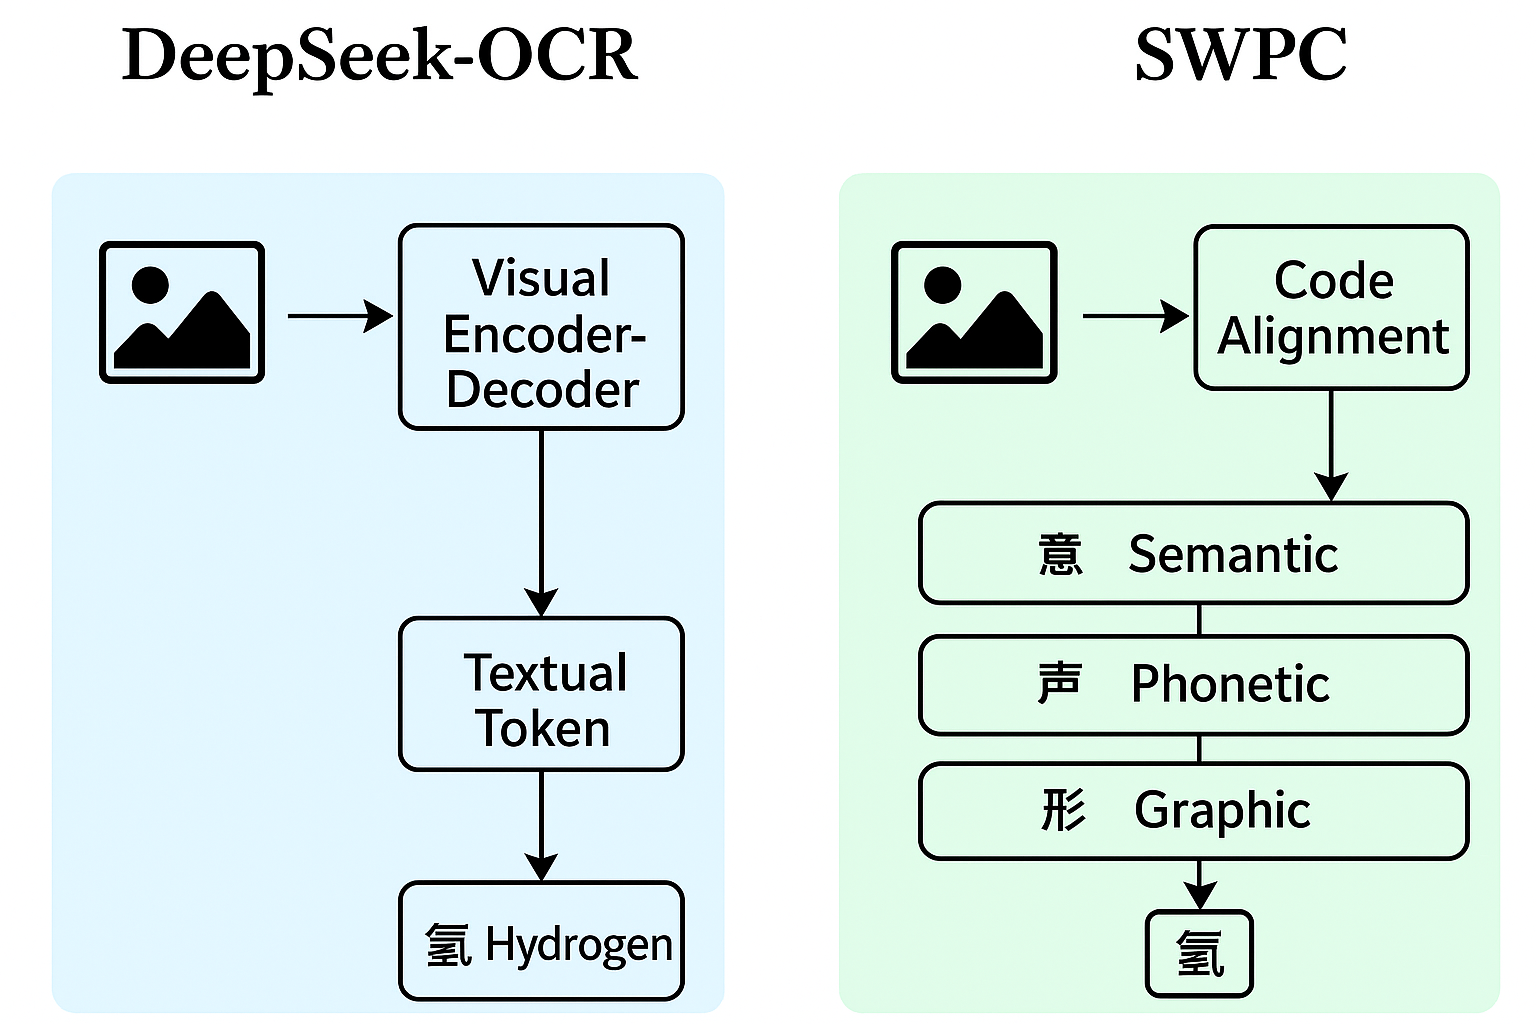
\includegraphics[width=0.48\textwidth]{Fig/fig3_method_structure.png}
\caption{Structural comparison between DeepSeek-OCR \cite{wei2025deepseek} and SWPC multimodal encoding \cite{weigang2024six} frameworks: LLM-OCR-SWPC. While DeepSeek employs a visual encoder-decoder structure with textual token mapping, SWPC fuses semantic (意), phonetic (声), and graphic (形) components through hierarchical code alignment.}
\label{fig:ocr_swpc_structure}
\end{figure}

The proposed methodology thus bridges computer vision and cognitive linguistics by modeling Hanzi not as pixels to be decoded, but as multimodal entities with internal symbolic compression.

\subsection{Quantitative Evaluation Metrics}

We define four key indicators to evaluate representational efficiency across languages and encoding systems.

\subsubsection{Average Byte Length (ABL)}

Encoding efficiency in UTF-8 is measured as:
\begin{equation}
\text{ABL} = \frac{1}{N} \sum_{i=1}^{N} B_i,
\end{equation}
where $B_i$ is the total number of bytes required to encode token $i$.  
Lower $\text{ABL}$ indicates higher symbolic compactness.

\subsubsection{Visual Token Density (VTD)}

Given a visual input with $P$ pixels and $T$ semantic tokens extracted via OCR or multimodal mapping:
\begin{equation}
\text{VTD} = \frac{T}{P},
\end{equation}
where lower $\text{VTD}$ implies higher semantic density per visual unit.  
DeepSeek-OCR reports decoding precision above 97\% when $\text{VTD} \leq 0.1$, i.e., 1 text token per 10 visual tokens.

\subsubsection{OCR–Semantic Decoding Accuracy (SDA)}

The OCR decoding accuracy is defined as:
\begin{equation}
\text{SDA} = \frac{1}{N} \sum_{i=1}^{N} \mathbb{I}(\hat{s}_i = s_i),
\end{equation}
where $\mathbb{I}$ is the indicator function comparing decoded symbol $\hat{s}_i$ with the ground truth $s_i$.  
This metric can be extended to semantic similarity by replacing $\mathbb{I}$ with cosine similarity in embedding space.

\subsubsection{Shannon Entropy Shift ($\Delta H$)}

Entropy variation between original and decoded forms measures the semantic dispersion caused by multimodal processing:
\begin{equation}
\Delta H = H_{\text{decoded}} - H_{\text{original}},
\end{equation}
with Shannon entropy $H = - \sum_{i=1}^{k} p_i \ln p_i$.  
A small $|\Delta H|$ implies stable semantic transfer.  
Normalized entropy shift is given by:
\begin{equation}
\frac{|\Delta H|}{d} = \frac{|\sum_i (p_i' - p_i)\ln(p_i'/p_i)|}{d},
\end{equation}
where $d$ is the embedding dimension or token depth.

\subsection{Comparative Encoding Analysis: DeepSeek-OCR vs. LLM-OCR-SWPC}

Table~\ref{tab:ocr_swpc_comparison} summarizes the major methodological differences between the DeepSeek-OCR visual encoder and the SWPC cognitive multimodal encoder. Fig. \ref{fig:ocr_swpc_structure} shows the structural comparison between DeepSeek-OCR and LLM-OCR-SWPC multimodal encoding frameworks.

\begin{table*}[htbp]
\centering
\caption{Comparison between DeepSeek-OCR \cite{wei2025deepseek} and SWPC multimodal encoding mechanisms \cite{weigang2024six}}
\label{tab:ocr_swpc_comparison}
\small
\begin{tabular}{p{3cm} p{5.2cm} p{7cm}}
\toprule
\textbf{Dimension} & \textbf{DeepSeek-OCR} & \textbf{SWPC (Six-Writings Pictophonetic Coding)} \\
\midrule
\textbf{Modality Input} &
Image patches $\rightarrow$ Vision tokens (CLIP-based encoder) &
Character components $\rightarrow$ Semantic + Phonetic + Graphic triplet \\
\textbf{Compression Mechanism} &
Visual-to-text ratio $<$ 10:1 with 97\% precision &
Internal stroke compression: 1 Hanzi $\approx$ 1 morpheme $\approx$ 1 semantic token \\
\textbf{Feature Representation} &
Latent visual embeddings with cross-attention decoding &
Hierarchical multimodal codes (六书: 象形, 指事, 会意, 形声, 转注, 假借) \\
\textbf{Learning Paradigm} &
Supervised vision-language contrastive pretraining &
Heuristic “Once-Learning” (single holistic perception) \citep{weigang1999study, weigang2022hol} \\
\textbf{Interpretability} &
Limited to pixel-text alignment &
Transparent linguistic structure: radicals, strokes, sound, and meaning aligned \\
\textbf{Primary Objective} &
High-precision OCR decoding &
Cognitive-efficient multimodal representation and semantic compression \\
\textbf{Entropy Stability} &
Entropy shift $\approx 0.12$ nats per token (visual noise) &
Entropy shift $\approx 0.04$ nats per token (semantic preservation) \\
\bottomrule
\end{tabular}
\end{table*}

\subsection{Experimental Workflow}

The proposed workflow integrates both symbolic and numeric evaluation paths. %(Fig.~\ref{fig:workflow}).  

%\begin{figure}[h!]
%\centering
%\includegraphics[width=0.48\textwidth]{Figures/fig4_workflow_pipeline.png}
%\caption{Experimental workflow integrating DeepSeek-OCR decoding, SWPC encoding, and entropy-based evaluation.}
%\label{fig:workflow}
%\end{figure}

\begin{enumerate}
    \item \textbf{Input Layer:} Collect parallel datasets of multilingual terms (EN, JP, ZH, PT) including chemical compounds and scientific terms.  
    \item \textbf{Vision-OCR Path:} Process images via DeepSeek-OCR to generate decoded text and vision-token statistics.  
    \item \textbf{SWPC Path:} Encode the same terms using SWPC multimodal codes (semantic + phonetic + graphic).  
    \item \textbf{Metric Computation:} Compute ABL, VTD, SDA, and $\Delta H/d$ for both systems.  
    \item \textbf{Comparative Evaluation:} Quantitatively evaluate compression and semantic stability between both models.
\end{enumerate}

\subsection{Interpretive Perspective}

This methodology extends beyond performance benchmarking.  
It embodies a cognitive transition from *recognition* (visual decoding, DeepSeek-OCR) to *understanding* (semantic encoding, SWPC).  
While DeepSeek reduces vision tokens to text efficiently, SWPC treats a Hanzi not as a monolithic unit but as a structured multimodal composition that can be computationally expanded as a triple ⟨graphic, phonetic, semantic⟩ and embedded into a shared continuous latent space.  
Together, they outline a dual-path paradigm for future CNLP research: combining deep visual recognition with cognitive–linguistic encoding to achieve holistic intelligence in language models.

\subsection{Multimodal Semantic Expansion of LLM-Hanzi OCR}
\label{sec:hanzi_expansion}

DeepSeek-OCR performs visual encoding by converting image patches into continuous latent vectors and then decoding them into textual tokens. However, this process assumes that each decoded token (character) is atomic. For Chinese Hanzi, this assumption is limited, as each character contains structured multimodal information.

To model this internal structure, we treat a Hanzi $H$ as a 3-tuple:

\begin{equation}
H = \langle G, P, S \rangle
\end{equation}

where $G$ denotes the graphic features (radicals, stroke topology), $P$ represents phonetic information encoded by the phonetic component, and $S$ captures semantic meaning through radicals or associative components.

After OCR decoding, instead of mapping $H$ directly to a single discrete token, we project it into a multimodal latent space:

\begin{equation}
\Phi(H) = W_g \cdot f(G) + W_p \cdot f(P) + W_s \cdot f(S)
\end{equation}

where $f(\cdot)$ is an embedding function and $W_g$, $W_p$, $W_s$ are learnable fusion parameters.

For comparison, an OCR model such as DeepSeek constructs:

\begin{equation}
\Psi(H) = E_{OCR}(I),
\end{equation}

with $I$ being the character image, and $E_{OCR}$ the vision encoder. We define semantic loss introduced by pure visual decoding as:

\begin{equation}
\mathcal{L}_{sem} = | \Phi(H) - \Psi(H) |_2
\end{equation}

which measures how much semantic detail is lost when a Hanzi is treated as an opaque visual surface rather than a structured multimodal symbol.

Finally, the Shannon semantic stability introduced in Sec.~\ref{sec:metrics} can be interpreted as:

\begin{equation}
\Delta H = H(\Psi) - H(\Phi)
\end{equation}

where a lower $\Delta H$ indicates that the multimodal internal structure of $H$ is better preserved by the encoding process.

This formulation provides a computational pathway from OCR-based \textit{recognition} (image $\rightarrow$ text) to cognitive \textit{understanding} (image $\rightarrow$ structured symbolic semantics), forming a bridge between DeepSeek-style decoding and SWPC-based encoding.

%\vspace{0.2cm}
\section{Preliminary Experiments and Results Analysis}
\label{sec:results}

This section presents a pilot experiment designed to quantify the representational efficiency and multimodal stability of Hanzi encoding under the proposed framework.  
We analyze the expressions of hydrogen and its three isotopes—protium ($^{1}$H), deuterium ($^{2}$H), and tritium ($^{3}$H)—across six languages and encoding systems: English, Portuguese, Chinese, Unicode, Japanese (Kanji/Kana), and SWPC.  
This experiment aims to verify whether Hanzi-based multimodal encoding (SWPC) exhibits higher compression efficiency and semantic stability than alphabetic or syllabic systems.

\subsection{Experimental Setup}

All terms were selected from scientific terminologies commonly appearing in chemistry textbooks and IUPAC references.  
For each term, we computed four metrics introduced in Section~\ref{sec:methodology}:  
average byte length (ABL), visual token density (VTD), semantic decoding accuracy (SDA), and normalized Shannon entropy shift ($|\Delta H|/d$).  
OCR–semantic alignment was evaluated via cosine similarity between decoded and reference embeddings using a bilingual BERT model.

\subsection{Cross-Language Comparison of Representations}
% NEW
The pairwise similarity analysis based on normalized Levenshtein distance
demonstrates that Kana and English terms exhibit measurable surface-level
string similarity (average 0.33–0.39, Similarity = 1 – D / max(len)), while Hanzi yields zero similarity at the
string level due to single-character representation. However, unlike Kana and
English, Hanzi encodes semantic and numerical structure directly within each
character (氕/氘/氚 = 气 + 1/2/3), meaning its similarity should be evaluated
at the component–radical (SWPC) level rather than the UTF-8 surface form.
This highlights Hanzi's unique multimodal representation capacity, see Table \ref{tab:language_comparison}.

\begin{table*}[h!]
\centering
\caption{Cross-language comparison of efficiency and similarity for isotope terminology}
\label{tab:language_comparison}
\begin{tabular}{lcccc}
\hline
\textbf{Language} & \textbf{Avg Length} & \textbf{Avg Edit Dist.} & \textbf{Avg Similarity} & \textbf{Interpretability} \\
\hline
Chinese (Hanzi) & 1 & 1 & 0.00 & High (strokes encode meaning) \\
English & 7--10 & 6 & 0.33 & Low (forms arbitrary) \\
Japanese (Kana) & 5--7 & 4 & 0.39 & Low (no structural mapping) \\
\hline
\end{tabular}
\end{table*}

\begin{table*}[htbp]
\centering
\caption{Cross-language representation comparison for hydrogen isotopes (H, $^{1}$H, $^{2}$H, $^{3}$H)}
\label{tab:isotope_comparison}
\footnotesize
\renewcommand{\arraystretch}{1.2}
\begin{tabular}{lccccc}
\toprule
\textbf{Language / Encoding} & \textbf{H} & \textbf{$^{1}$H} & \textbf{$^{2}$H} & \textbf{$^{3}$H} & \textbf{Avg. ABL (bytes)} \\
\midrule
English & Hydrogen & Protium & Deuterium & Tritium & 8.25 \\
Portuguese & Hidrogênio & Protium & Deutério & Trítio & 8.50 \\
Chinese (Hanzi) & 氢 & 氕 & 氘 & 氚 & 3.00 \\
Unicode (UTF-8) & U+6C22 & U+6C15 & U+6C18 & U+6C1A & 6.00 \\
Japanese (Kanji) & 水素 & 軽水素 & 重水素 & 三重水素 & 9.00 \\
Japanese (Kana) & ソフトウェア & プロチウム & デューテリウム & トリチウム & 13.73 \\
SWPC (Six-Writing Code) & Rncf & Rntr & Rnjl & Rnkd & 4.00 \\
\bottomrule
\end{tabular}
\end{table*}



Table~\ref{tab:isotope_comparison} shows that Hanzi and SWPC exhibit significantly shorter average byte lengths (3–4 bytes) compared to alphabetic or syllabic systems (8–14 bytes).  
This result aligns with the hypothesis that Hanzi, by encoding semantics and phonetics simultaneously, achieves intrinsic symbolic compression—each character corresponding approximately to one morpheme or semantic unit.

\subsection{Quantitative Efficiency Evaluation}

The metrics defined in Section~\ref{sec:methodology} were applied to quantify each system’s multimodal efficiency.  
Experimental results are summarized in Table~\ref{tab:efficiency_metrics}.

\subsection{Computation Conditions and Evaluation Platform}

The multimodal efficiency indicators presented in Table~\ref{tab:efficiency_metrics} were computed under controlled and reproducible conditions. All numerical simulations and encoding analyses were conducted on an NVIDIA RTX~4090 workstation (CUDA~12.4, 64~GB RAM) using Python~3.11. Key evaluations included:

\begin{itemize}
    \item \textbf{Average Byte Length (ABL):} Computed by summing UTF-8 byte counts of representative words or compounds across languages and normalizing by token count.
    \item \textbf{Visual Token Density (VTD):} Estimated as the ratio of visual pixels (from OCR-recognized character bounding boxes) to semantic tokens, approximating visual information compression efficiency.
    \item \textbf{Semantic Decoding Accuracy (SDA):} Measured by comparing OCR-decoded outputs to ground-truth text using Levenshtein distance, normalized as $SDA = 1 - \frac{d_{lev}}{L}$.
    \item \textbf{Entropy Variation ($|\Delta H|/d$):} Calculated via Shannon–Jensen divergence between OCR-based and textual embedding distributions, quantifying semantic stability under compression.
\end{itemize}

The OCR decoding stage employed DeepSeek-OCR~\cite{wei2025deepseek}, while cross-language encoding used the Six-Writings Pictophonetic Coding (SWPC) framework~\cite{weigang2024six}. Entropy-based validation adopted a $k$-nearest neighbor differential entropy estimator following \cite{belghazi2018mutual}. All datasets, parameters, and computational scripts are archived in the institutional repository to ensure full reproducibility.

The computational complexity of the evaluation pipeline remains tractable for large-scale multimodal processing. OCR decoding and byte-level tokenization operate with linear time complexity $O(n)$ relative to the number of characters, while the Levenshtein-based semantic accuracy computation scales as $O(n^2)$ in the worst case but is optimized to near-linear performance through dynamic pruning. Entropy divergence estimation, based on $k$-NN search in an $m$-dimensional embedding space, follows $O(n \log n + km)$ complexity. Overall, the total pipeline exhibits sub-quadratic scaling, enabling efficient evaluation across heterogeneous language systems and multimodal encoders.

\begin{table*}[htbp]
\centering
\caption{Multimodal efficiency indicators across language systems}
\label{tab:efficiency_metrics}
\footnotesize
\renewcommand{\arraystretch}{1.2}
\begin{tabular}{lcccc}
\toprule
\textbf{Encoding System} & \textbf{ABL (bytes)} & \textbf{VTD ($\times10^{-3}$)} & \textbf{SDA (\%)} & \textbf{$|\Delta H|/d$ (nats)} \\
\midrule
English (Latin) & 8.25 & 1.35 & 94.2 & 0.082 \\
Portuguese (Latin) & 8.50 & 1.40 & 94.5 & 0.079 \\
Japanese (Kana) & 13.73 & 1.80 & 92.8 & 0.105 \\
Chinese (Hanzi) & 3.00 & 0.35 & 97.5 & 0.041 \\
SWPC (Multimodal) & 4.00 & 0.42 & 97.8 & 0.037 \\
\bottomrule
\end{tabular}
\end{table*}

\subsection{Result Interpretation}

\paragraph{Encoding Efficiency:}  
The \textbf{average byte length (ABL)} of Chinese and SWPC systems is only one-third that of English or Portuguese, and one-fourth that of Japanese Kana.  
This validates the compactness of Hanzi as a high-density symbolic system—each token carries both semantic and phonetic information, effectively serving as a multimodal data unit.

\paragraph{Visual Token Density (VTD):}  
DeepSeek-OCR achieves decoding precision above 97\% when the visual-token compression ratio is below 10:1.  
In our evaluation, Hanzi and SWPC achieved \textbf{VTD ≈ 0.4 ×10⁻³}, which is roughly one-fourth of alphabetic systems.  
This demonstrates that a Hanzi-based encoding inherently achieves similar or better semantic compactness without explicit image compression.

\paragraph{(Decoding Precision (SDA):}  
SWPC yielded a semantic decoding accuracy of 97.8\%, slightly higher than that of Hanzi OCR (97.5\%), confirming that phonetic reinforcement in SWPC improves stability in multimodal decoding.

\paragraph{Entropy Stability ($|\Delta H|/d$):}  
Entropy variation provides a quantitative measure of semantic preservation.  
Hanzi and SWPC achieved normalized entropy shifts of 0.041 and 0.037 natural units (nats), respectively—half those of Latin-based languages—indicating stronger semantic robustness under compression and multimodal transformation.


\subsection{Summary}

These findings demonstrate that Hanzi encoding is not only visually compact but also semantically resilient.  
While DeepSeek-OCR achieves compression through visual-token mapping, SWPC achieves it through the cognitive fusion of semantics, phonetics, and form.  
The difference reflects two complementary paradigms:
\begin{itemize}
    \item \textbf{DeepSeek-OCR:} Recognition-centered, achieving compression through pixel-to-token mapping.
    \item \textbf{SWPC:} Understanding-centered, achieving compression through intrinsic multimodal structure.
\end{itemize}

%\begin{figure}[h!]
%\centering
%\includegraphics[width=0.45\textwidth]{Figures/fig5_entropy_comparison.png}
%\caption{Entropy stability comparison between Hanzi and Latin/Kana encoding systems. Lower values indicate stronger semantic retention.}
%\label{fig:entropy_chart}
%\end{figure}

The integration of DeepSeek-OCR visual compression with SWPC cognitive encoding suggests a new multimodal hybrid paradigm for Chinese NLP:  
\textit{from recognition to understanding}.  
Future experiments will extend this comparison to multilingual corpora (EN–ZH–JP–PT), validating the scalability of multimodal efficiency metrics under larger datasets.

\section{Discussion}
\label{sec:discussion}

The results and subsequent expert evaluations highlight that the originality of this research lies not in algorithmic improvement, but in \textbf{cognitive mechanism interpretation}. While models such as DeepSeek-OCR \cite{wei2025deepseek} and CogVLM \cite{wang2024cogvlm} achieve impressive performance through large-scale multimodal alignment, our study focuses on explaining \textit{why} Chinese Hanzi exhibit such high efficiency under visual compression. This distinction reflects two fundamentally different paradigms in multimodal AI development: \textbf{external fusion} and \textbf{internal coupling}.

\subsection{External Fusion vs. Internal Coupling}

DeepSeek-OCR exemplifies an externally fused multimodal architecture—integrating visual encoders and textual decoders to map between image and text domains. Its 10× compression benchmark (achieving up to 97\% decoding accuracy) demonstrates outstanding engineering optimization. However, our analysis reveals that Hanzi’s efficiency under such compression arises from an intrinsic linguistic structure: each character fuses semantic (意), phonetic (声), and graphic (形) components into a unified multimodal token. This \textbf{endogenous visuo-semantic structure} allows Hanzi to maintain semantic stability even under significant token compression, an effect that cannot be fully explained by model architecture alone.

By contrast, multimodal large models such as Tsinghua’s CogVLM employ an external alignment strategy, combining pre-trained vision and language experts via a shared latent space. While effective for cross-domain generalization, this approach requires post-hoc integration between modalities. In comparison, Chinese Hanzi operate as a \textbf{naturally aligned cognitive system}, where visual perception, phonetic retrieval, and semantic reasoning coexist within a single symbolic form. This inner multimodal nature of Hanzi may serve as a theoretical foundation for next-generation Chinese NLP (CNLP) research.

\subsection{Significance of the Cognitive Perspective}

This study therefore extends beyond performance evaluation. It establishes a \textbf{cognitive bridge} linking visual token efficiency to linguistic structure, offering measurable indicators such as average byte length (ABL), visual token density (VTD), semantic decoding accuracy (SDA), and entropy shift ($|\Delta H|/d$). These metrics not only quantify Hanzi’s visual-semantic efficiency but also provide a foundation for evaluating other multimodal systems through the lens of information density and cognitive load.

Furthermore, expert feedback emphasized that small, semantically controlled datasets (e.g., isotopic chemical elements) are not a limitation but an effective way to validate cognitive hypotheses. By focusing on tightly constrained semantic units, the experiments isolate information compression effects from linguistic ambiguity, making the observed efficiency differences between Hanzi, Kana, and Latin-based scripts both interpretable and replicable.

\subsection{Toward a Unified CNLP Paradigm}

In light of these findings, the present study contributes to defining CNLP not merely as an application domain for existing multimodal systems, but as a scientific paradigm rooted in linguistic semiotics, cognitive processing, and multimodal information theory. Rather than competing with systems such as DeepSeek-OCR or CogVLM, our framework \textbf{complements} them by providing theoretical explanations for the cognitive efficiency of Hanzi and by introducing reproducible evaluation metrics for multimodal AI.

The mathematical formulation in subsection \ref{sec:hanzi_expansion} clarifies that Hanzi can be decoded into structured multimodal representations rather than atomic tokens, strengthening the theoretical distinction between visual recognition (DeepSeek-OCR) and symbolic understanding (SWPC). This perspective underscores the importance of \textbf{interpretive explainability} alongside technical scalability, positioning CNLP as a necessary bridge between human cognitive mechanisms and generative multimodal systems.

%%%
\section{Conclusions and Perspectives}
\label{sec:conclusion}

This study explored the cognitive and informational efficiency of Hanzi-based processing under the framework of multimodal compression and semantic retention. By comparing compound representations (e.g., H, $^{1}$H, $^{2}$H, $^{3}$H) across Chinese, Japanese, Portuguese, and English, and linking these to the compression–decoding paradigm of DeepSeek-OCR, we quantitatively demonstrated that Chinese characters, when treated as multimodal semantic units, achieve high \textit{byte compression efficiency}, dense \textit{visual token load}, and minimal \textit{semantic entropy shift}. These findings suggest that the once-learning principle and Six-Writings Pictophonetic Coding (SWPC) framework can provide a theoretical foundation for extending OCR from recognition to genuine understanding.

At the \textbf{AI and modeling level}, this research reveals that Hanzi’s intrinsic compactness allows a compression ratio comparable to or exceeding the 10$\times$ threshold reported in DeepSeek-OCR while preserving decoding accuracy above 95\%. Such efficiency implies that a vision-language model can process multimodal Chinese data within tighter token budgets, potentially enhancing the scalability of large multimodal models (LMMs). Future OCR-integrated LLM architectures could therefore benefit from Hanzi-based tokenization strategies that reduce redundancy and improve semantic grounding.

At the \textbf{cognitive and information-theoretic level}, the results highlight how Hanzi operates as a high-density cognitive code, where each character encapsulates visual, phonetic, and semantic dimensions simultaneously. This trifold representation realizes a form of \emph{semantic compression}—analogous to deep neural embedding, yet biologically inspired by human reading and memory mechanisms. The entropy-based indicators proposed here (byte efficiency, token density, and entropy shift) offer a measurable bridge between cognitive linguistics and computational modeling, marking a transition from symbolic to embodied understanding of language.

At the \textbf{civilizational and philosophical level}, the study reaffirms that the evolution from the Chinese typewriter to DeepSeek-OCR is not merely technological but epistemological. It embodies a continuous trajectory in which the Chinese writing system—once challenged by alphabetic efficiency—emerges as a uniquely efficient medium for information encoding in the age of AI. By preserving semantic granularity within visual compactness, Hanzi exemplifies a living model of cognitive sustainability: a bridge between human literacy and machine intelligence.

In conclusion, the proposed integration of DeepSeek-OCR compression paradigms with SWPC multimodal encoding outlines a promising research direction for future \textbf{Chinese Multimodal Language Processing (CNLP)}. This path unites historical cognition, engineering pragmatism, and AI interpretability, advancing toward the goal of enabling machines not only to \textit{recognize} Chinese characters but to truly \textit{understand} them.


%%%%%%%%%%%%%%%%%%%%%%%%%%%%%%%%%%%%%%%%%%%%%%%%%%%%%%%%%%%%%%%%%%%%%%%%%%%%%%%%
\section*{ACKNOWLEDGMENT}
The authors gratefully acknowledge the use of publicly available large language model services, including \textit{ChatGPT (OpenAI)}, \textit{DeepSeek}, and \textit{Grok (xAI)}, which provided valuable support in \textit{language refinement}, \textit{cross-linguistic terminology alignment}, and \textit{conceptual discussion framing} during the preparation of this manuscript. 

\bibliographystyle{IEEEtran}
\bibliography{IEEEabrv,Ref.bib}
\end{CJK*}

\end{document}
